\documentclass[10pt]{article}
\usepackage[margin=1in]{geometry}
%\addtolength{\oddsidemargin}{-.1in} 
\usepackage{amsmath,amsthm,amssymb}
\usepackage{bm}
\usepackage{enumitem}
\usepackage{array}
\usepackage{lipsum}
\usepackage[]{units}
\usepackage{relsize}
\usepackage{verbatim}

\usepackage{tikz}
\usetikzlibrary{positioning}
\usepackage{graphicx}
\usepackage{xfrac}

\setenumerate{listparindent=\parindent}

\newcommand{\Q}{\mathbf{Q}}
\newcommand{\Z}{\mathbf{Z}}
\newcommand{\R}{\mathbf{R}}
\DeclareMathOperator*{\dom}{dom}
\DeclareMathOperator*{\Aut}{Aut}
\DeclareMathOperator*{\Ann}{Ann}
\DeclareMathOperator*{\Tor}{Tor}
\DeclareMathOperator*{\Gal}{Gal}
\DeclareMathOperator*{\Hom}{Hom}
\DeclareMathOperator*{\End}{End}
\DeclareMathOperator*{\im}{Im}
\renewcommand{\bar}{\overline}

\usepackage{fancyhdr} % Required for custom headers 
%\usepackage{lastpage} % Required to determine the last page for the footer

\pagestyle{fancy}
\lhead{Math 114 (HW11)}
\chead{Michael Knopf (24457981)}
\rhead{April $30^\text{th}$, 2015}
\lfoot{}
\cfoot{}
\rfoot{}
%\rfoot{Page\ \thepage\ of\ \pageref{LastPage}}
\renewcommand\headrulewidth{0.4pt}
%\renewcommand\footrulewidth{0.4pt}

\begin{document}

In all exercises, you may assume $R$ is a commutative ring with identity where $1 \neq 0$.

\begin{enumerate}

\item (Exercise 14 in DF \S 10.4.) Let $I$ be an arbitrary nonempty index set, and for each $i \in I$ let $N_i$ be an $R$-module.  Let $M$ be an $R$-module.  Prove that there is an $R$-module isomorphism
$$
M \otimes_R \left( \bigoplus_{i \in I} N_i \right) \cong \bigoplus_{i \in I} (M \otimes_R N_i).
$$

\begin{proof}

Define a map $f: M \times \left( \bigoplus_{i \in I} N_i \right) \rightarrow \bigoplus_{i \in I} (M \otimes_R N_i)$ by $(m, \prod n_i) \mapsto \prod m \otimes n_i$.  Observe that $f$ is bilinear: for any $r_1, r_2 \in R, m_1, m_2 \in M,$ and $\prod x_i, \prod y_i \in \oplus_{i \in I} N_i$, we have
\begin{align*}
f((r_1m_1 + r_2m_2, \prod x_i))
&=
\prod(r_1m_1 + r_2m_2) \otimes x_i
\\
&= r_1 \prod(m_1 \otimes x_i) + r_2 \prod (m_2 \otimes x_i)
\\
&= r_1 f(m_1, x_i) + r_2 f(m_2, x_i)
\\
f((m_1, r_1\prod x_i + r_2 \prod y_i)
&=
m_1 \otimes (r_1\prod x_i + r_2 \prod y_i)
\\
&= \prod m_1 \otimes (r_1 x_i + r_2 y_i)
\\
&= r_1 \prod m_1 \otimes x_i + r_2 \prod m_1 \otimes y_i
\\
&= r_1 f(m_1, \prod x_i) + r_2 f(m_1, \prod y_i)
\end{align*}
therefore, by the universal property of tensor product (the version from Corollary 12), $f$ induces a unique $R$-module homomorphism $\varphi : M \otimes_R \left( \bigoplus_{i \in I} N_i \right) \rightarrow \bigoplus_{i \in I} (M \otimes_R N_i)$ defined by $(m \otimes \prod n_i) \mapsto \prod(m \otimes n_i)$.


\begin{comment}
Next, for each $i \in I$ define a map $g_i: M \times N_i \rightarrow M \otimes_R (\oplus_{i \in I} N_i)$ by $(m, n) \mapsto m \otimes \prod n_j$ where $n_j = n$ if $j = i$ and $n_j = 0$ otherwise.  Observe that $g_i$ is bilinear: for each $r_1, r_2 \in R, m_1, m_2 \in M$, and $x,y \in N_i$, again define $x_j = x$ if $j=i$ and $x_j = 0$ if $j \neq i$ (and define $y_j$ similarly).  We have
\begin{align*}
g_i(r_1m_1 + r_2m_2, x)
&=
(r_1m_1 + r_2m_2) \otimes \prod x_j
\\
&= r_1 \left( m_1 \otimes \prod  x_j \right) + r_2 \left( m_2 \otimes \prod x_j \right)
\\
&= r_1 g_i(m_1, x) + r_2 g_i(m_2, x)
\\
g_i(m_1, r_1 x + r_2 y)
&=
m_1 \otimes \prod n_j \text{ where } n_j = r_1x + r_2y \text{ if } j = i \text{ and } 0 \text{ otherwise}
\\
&= r_1 \left( m_1 \otimes \prod x_j \right) + r_2 \left( m_1 \otimes \prod y_j \right)
\\
&= r_1 g(m_1, x) + r_2 g(m_1, y)
\end{align*}
therefore each $g_i$ induces an $R$-module homomorphism $\psi_i : M \otimes_R N_i \rightarrow M \otimes_R (\oplus_{i \in I} N_i)$ defined by $\psi_i ( m \otimes n) = m \otimes \prod n_j$, where $n_j$ is defined as it was before.

By the universal property of direct sum, there is a unique $R$-module homomorphism $\psi : \oplus_{i \in I} (M \otimes N_i) \rightarrow M \otimes (\oplus_{i \in I} N_i)$ such that $\psi \circ \iota_i = \psi_i$ for each $i \in I$.  We will now show that $\psi$ is the inverse of $\varphi$, thus giving that $\varphi$ is an isomorphism.

Let $m \otimes \prod n_i \in M \otimes_R (\oplus_{i \in I} N_i)$, so that $n_i \in N_i$ for each $i \in I$.

Note that there are only finitely many $i \in I$ for which $n_i \neq 0$, so $\prod_{i \in I} m \otimes n_i = \sum\limits_{\{i  : n_i \neq 0 \}} \iota_i(m \otimes n_i)$ is a sum of finitely many terms.  We have

\begin{align*}
\psi \circ \varphi \left( m \otimes \prod n_i \right)
&=
\psi \left( \prod m \otimes n_i \right)
\\
&= \psi \left( \sum\limits_{\{i  : n_i \neq 0 \}} \iota_i(m \otimes n_i) \right)
\\
&= \sum\limits_{\{i  : n_i \neq 0 \}} \psi \circ \iota_i (m \otimes n_i)
\\
&= \sum\limits_{\{i  : n_i \neq 0 \}} \psi_i (m \otimes n_i)
\\
&= \sum\limits_{\{i  : n_i \neq 0 \}} m \otimes \prod n_j
\\
&=  m \otimes \sum\limits_{\{i  : n_i \neq 0 \}} \prod n_j
\\
&= m \otimes \prod
\end{align*}
\end{comment}


Next, for each $i \in I$ define a map $g_i: M \times N_i \rightarrow M \otimes_R (\oplus_{i \in I} N_i)$ by $(m, n) \mapsto m \otimes \iota_i (n)$ where $\iota_i$ is the natural inclusion of $N_i$ into $\oplus_{i \in I} N_i$.  Recall that $\iota_i$ is an $R$-module homomorphism.  Observe that $g_i$ is bilinear: for each $r_1, r_2 \in R, m_1, m_2 \in M$, and $x,y \in N_i$, we have
\begin{align*}
g_i(r_1m_1 + r_2m_2, x)
&=
(r_1m_1 + r_2m_2) \otimes \iota_i(x)
\\
&= r_1 \left( m_1 \otimes \iota_i(x) \right) + r_2 \left( m_2 \otimes \iota_i(x) \right)
\\
&= r_1 g_i(m_1, x) + r_2 g_i(m_2, x)
\\
g_i(m_1, r_1 x + r_2 y)
&=
m_1 \otimes \iota_i(r_1 x + r_2 y)
\\
&= r_1 \left( m_1 \otimes \iota_i(x) \right) + r_2 \left( m_1 \iota_i(y) \right)
\\
&= r_1 g(m_1, x) + r_2 g(m_1, y)
\end{align*}
therefore each $g_i$ induces a unique $R$-module homomorphism $\psi_i : M \otimes_R N_i \rightarrow M \otimes_R (\oplus_{i \in I} N_i)$ satisfying $\psi_i ( m \otimes n) = m \otimes \iota_i(n)$.

By the universal property of direct sum, there is a unique $R$-module homomorphism $\psi : \oplus_{i \in I} (M \otimes N_i) \rightarrow M \otimes (\oplus_{i \in I} N_i)$ such that $\psi \circ \hat{\iota}_i = \psi_i$ for each $i \in I$, where $\hat{\iota}_i$ is the inclusion of $M \otimes_R N_i$ into $\oplus_{j \in I} (M \otimes_R N_j)$.

We will now show that $\psi$ is the inverse of $\varphi$, thus giving that $\varphi$ is an isomorphism.  Let $m \otimes \prod n_i \in M \otimes_R (\oplus_{i \in I} N_i)$, where $n_i \in N_i$ for each $i \in I$.  Note that there are only finitely many $i \in I$ for which $n_i \neq 0$, so $\prod_{i \in I} m \otimes n_i = \sum\limits_{\{i  : n_i \neq 0 \}} \hat{\iota_i}(m \otimes n_i)$ is a sum of finitely many terms.  We have

\begin{align*}
\psi \circ \varphi \left( m \otimes \prod n_i \right)
&=
\psi \left( \prod m \otimes n_i \right)
\\
&= \psi \left( \sum\limits_{\{i  : n_i \neq 0 \}} \hat{\iota_i} (m \otimes n_i) \right)
\\
&= \sum\limits_{\{i  : n_i \neq 0 \}} \psi \circ \hat{\iota_i} (m \otimes n_i)
\\
&= \sum\limits_{\{i  : n_i \neq 0 \}} \psi_i (m \otimes n_i)
\\
&= \sum\limits_{\{i  : n_i \neq 0 \}} m \otimes \iota_i(n_i)
\\
&=  m \otimes \sum\limits_{\{i  : n_i \neq 0 \}} \iota_i (n_i)
\\
&= m \otimes \prod n_i
\end{align*}
so $\psi$ is a left inverse of $\varphi$.

Next, let $\prod m_i \otimes n_i \in \oplus_{i \in I} (M \otimes_R N_i)$, where $m_i \in M, n_i \in N_i$ for each $i \in I$.  We have
\begin{align*}
\varphi \circ \psi \left( \prod m_i \otimes n_i \right)
&=
\varphi \circ \psi \left( \sum_{\{ i : m_i \otimes n_i \neq 0 \}} \hat{\iota}_i(m_i \otimes n_i) \right)
\\
&= \varphi \left( \sum_{\{ i : m_i \otimes n_i \neq 0 \}} \psi_i(m_i \otimes n_i) \right)
\\
&= \varphi \left( \sum_{\{ i : m_i \otimes n_i \neq 0 \}} m_i \otimes \iota_i(n_i) \right)
\\
&= \sum_{\{ i : m_i \otimes n_i \neq 0 \}} \varphi \left( m_i \otimes \iota_i(n_i) \right)
\\
&= \sum_{\{ i : m_i \otimes n_i \neq 0 \}} \hat{\iota}_i \left( \prod m_i \otimes n_i \right)
\\
&= \prod m_i \otimes n_i
\end{align*}
therefore $\psi$ is also a right inverse of $\varphi$, so $\varphi$ is an isomorphism.
\end{proof}

\item (Exercise 16 in DF \S 10.4.) Let $I$ and $J$ be ideals of $R$, so that $R/I$ and $R/J$ are naturally $R$-modules.

(a) Prove that every element of $R/I \otimes_R R/J$ can be written as a simple tensor of the form $\overline{1_R} \otimes \overline{r}$, where $r \in R$ and the bar in the left (resp. right) factor denotes the equivalence class modulo $I$ (resp. modulo $J$).

\begin{proof}
Every element of $R/I \otimes_R R/J$ can be written as $\sum_{i=1}^n \bar{x_i} \otimes \bar{y_i}$ for some $n$, where $x_i, y_i \in R$ for each $i \in \{1, \dots , n \}$.  Using the natural action of $R$ on $R/I \otimes_R R/J$, we have
$$
\sum_{i=1}^n \bar{x_i} \otimes \bar{y_i} = \sum_{i=1}^n \bar{1_R} \cdot x_i \otimes y_i \cdot \bar{1_R} = \sum_{i=1}^n \bar{1_R} \otimes (x_iy_i) \cdot \bar{1_R} = \sum_{i=1}^n \bar{1_R} \otimes \bar{x_i y_i} = \bar{1_R} \otimes \sum_{i=1}^n  \bar{x_i y_i} = \bar{1_R} \otimes \bar{\sum_{i=1}^n  x_i y_i}
$$
hence the result follows.
\end{proof}

(b) Prove that there is an $R$-module isomorphism $R/I \otimes_R R/J \cong R/(I+J)$ mapping $\overline{r} \otimes \overline{r'}$ to $\overline{rr'}$ (where $r, r' \in R$ and the bars denote the equivalence class modulo $I$, $J$, and $I+J$ respectively).  (Recall that $I+J$ denotes the ideal generated by the set $I \cup J$, or equivalently the set of all elements $a+b$ where $a \in I$ and $b \in J$.)

\begin{proof}
First, we need to show that the given map $\varphi$ is well-defined.  It is not enough to check that $\varphi(\bar{1}_R \otimes \bar{x}) = \varphi(\bar{1}_R \otimes \bar{y})$ when $x-y \in J$, since this is not equivalent to $\bar{1}_R \otimes \bar{x} = \bar{1}_R \otimes \bar{y}$.  For instance, in $\Z / 2\Z \otimes_{\Z} \Z / 3\Z = 0$ we have $\bar{1} \otimes \bar{1} = \bar{0} = \bar{1} \otimes \bar{2}$, even though $1 - 2 \not \in 3\Z$.  So we will again invoke the universal property.

Let $f: R/I \times R/J \rightarrow R/(I+J)$ be defined by $f(\bar{x},\bar{y}) = \bar{xy}$.  First, we will show that $f$ is well-defined.  Suppose $x - s \in I$ and $y - r \in J$.  Then $xy \in I$ and $sr \in J$ simply because $x,s \in R$, and $I+J$ is an $R$-module.  Thus $xy - rs \in I + J$, so $f(\bar{x},\bar{y}) = \bar{xy} = \bar{rs} = f(\bar{r},\bar{s})$.

Now, we will show that $f$ is bilinear.  For any $r,s,x,y,z \in R$, we have
$$
f(\bar{rx + sy},\bar{z}) = \bar{(rx+sy)z} = r \cdot \bar{xz} + s \cdot \bar{yz} = rf(\bar{x},\bar{z}) + sf(\bar{y},\bar{z})
$$
Since $R$ is commutative and $f$ is symmetric in its two arguments, linearity holds in the second component as well.  Thus $f$ induces an $R$-module homomorphism $R/I \otimes R/J \rightarrow R/(I+J)$, which is precisely $\varphi$.  Thus $\varphi$ is a well-defined homomorphism.

To see that $\varphi$ is injective, let $\bar{1}_R \otimes \bar{x} \in \ker (\varphi)$.  Then $1_R \cdot x = x \in I + J$, so $x = i + j$ for some $i \in I, j \in J$.  Thus $$\bar{1}_R \otimes \bar{x} = \bar{1}_R \otimes \bar{i + j} = \bar{1}_R \otimes \bar{i} + \bar{1}_R \otimes \bar{j} = \bar{i} \otimes \bar{1}_R + \bar{1}_R \otimes \bar{j} = \bar{0_R} \otimes \bar{1}_R + \bar{1}_R \otimes \bar{0_R} = 0.$$
Since $\varphi$ is a group homomorphism, and its kernel is $0$, it must be injective.

$\varphi$ is clearly surjective, since for any $x + (I+J) \in R/(I+J)$ we have $\varphi((1_R + I) \otimes (x + J)) = (1_R \cdot x) + (I+J) = x + (I + J)$.  Thus $\varphi$ is an isomorphism.
\end{proof}

\item (Exercise 18 in DF \S 10.4.) Suppose $R$ is an integral domain and $I$ is a principal ideal in $R$.  Prove that the $R$-module $I \otimes_R I$ has no nonzero torsion elements; i.e., if $r \in R \backslash \{0\}$ and $m \in I \otimes_R I$ satisfy $rm=0$, then $m=0$.

\begin{proof}
Let $I = (a)$, so that every element of $I$ is of the form $ra$ for some $r \in R$.  First, note that every tensor is of the form $\sum_i r_i a \otimes s_i a = \left(\sum_i r_is_i \right) \cdot (a \otimes a) = r \cdot (a \otimes a)$.  It is natural to guess that $I \otimes_R I \cong R$.

Define $f : I \times I \rightarrow R$ by $(ra,sa) \mapsto rs$.  Check that $f$ is bilinear: for any $c,d,r,s,t \in R$, we have
\begin{align*}
f(c(ra) + d(sa),ta)
&=
f((cr + ds)a, ta)
\\
&= (cr+ds)t
\\
&= c(rt) + d(st)
\\
&= cf(r,t) + df(s,t).
\end{align*}
Again, since $f$ is symmetric in its arguments we know it is linear in its second component as well.  So $f$ is bilinear, and thus induces a unique $R$-module homomorphism $\varphi: I \otimes_R I \rightarrow R$ such that $\varphi(ra \otimes sa) = rs$.  Since every tensor is of the form $r \cdot (a \otimes a)$, $\varphi$ is equivalently defined by $\varphi(r \cdot (a \otimes a)) = r$.

Clearly the map $\psi: R \rightarrow I \otimes_R I$ given by $r \mapsto r \cdot (a \otimes a)$ is a homomorphism and both a left and right inverse of $\varphi$:
\begin{align*}
\psi(x + ry) &= (x+ry) \cdot (a \otimes a) = x \cdot (a \otimes a) + r \cdot (y \cdot (a \otimes a)) = \psi(x) + r \psi(y)
\\
\varphi \circ \psi (r) &= \varphi(r \cdot (a \otimes a)) = r
\\
\psi \circ \varphi(r \cdot (a \otimes a)) &= \psi(r) = r \cdot (a \otimes a)
\end{align*}
Thus $\varphi$ is an isomorphism.

The action of $R$ on itself is simply multiplication in $R$, thus $R$ being torsion free is equivalent to it being an integral domain.  Therefore, $R$ is torsion free and so $I \otimes_R I$ must also be torsion free.
\end{proof}

\item (Exercise 19 in DF \S 10.4.) Let $I = (2,X)$ be the ideal generated by $2$ and $X$ in the ring $R = \mathbf{Z}[X]$, as in Exercise 17 (assigned on HW10).  Show that the nonzero element $2 \otimes X - X \otimes 2$ in $I \otimes_R I$ is a torsion element.  Show in fact that $2 \otimes X - X \otimes 2$ is annihilated by both $2$ and $X$, and that the submodule of $I \otimes_R I$ generated by $2 \otimes X - X \otimes 2$ is isomorphic to $R/I$.

\begin{proof}
\begin{align*}
2(2 \otimes x - x \otimes 2) &= (2 \otimes 2x - 2x \otimes 2) = (2x \otimes 2 - 2x \otimes 2) = 0
\\
x(2 \otimes x - x \otimes 2) &= (2x \otimes x - x \otimes 2x) = (2x \otimes x - 2x \otimes x) = 0
\end{align*}
thus $(2 \otimes x - x \otimes 2)$ is annihilated by both $2$ and $x$.  The only reason we could not do this before (in hw 10) was that $(2 \otimes x)$ cannot be written as $2(1 \otimes x)$, since $1 \not \in I$.

This implies that both $2$ and $x$ annihilate the submodule $A$ of $I \otimes_R I$ generated by $2 \otimes x - x \otimes 2$: in general, let $S$ be a commutative ring, let $\{v\}$ a basis for an $S$-module $V$, and suppose $a \in S$ annihilates $v$.  Any element of $V$ is of the form $sv$ for some $s \in S$, so we have
$$
a(sv) = (as)v = (sa)v = s(av) = s(0) = 0
$$
thus $a$ is contained in the annihilator of $V$.

Furthermore, this implies that $I$ is contained in the annihilator of $A$:  In homework 7, problem 5, we were allowed to take for granted the result of exercise 9 from section 10.1, which states that the annihilator of $A$ is an ideal.  This would be easy to show anyway, since the annihilator of a module is the kernel of the homomorphism $r \mapsto rx$, thus is an ideal.  Since $2$ and $x$ annihilate $A$, the annihilator of $A$ must contain the ideal generated by $2$ and $x$.  So $I$ annihilates $A$.

Define a map $\varphi : R \rightarrow A$ by $r(x) \mapsto r(x) \cdot (2 \otimes x - x \otimes 2)$.  $\varphi$ is clearly an $R$-module homomorphism:
\begin{align*}
\varphi(p(x) + r(x)q(x))
&=
p(x) + r(x)q(x)(2 \otimes x - x \otimes 2)
\\
&= p(x)(2 \otimes x - x \otimes 2) + r(x)(q(x)(2 \otimes x - x \otimes 2))
\\
&= \varphi(p(x)) + r(x) \cdot \varphi(q(x))
\end{align*}
Since $I$ annihilates $A$, it is contained in the kernel of $\varphi$.  We will now show that $I$ is \emph{precisely} this kernel.  Suppose $p(x) \in \Z[x]$, but $p(x) \not \in I$.  Then $p(x)$ has an odd constant term, thus can be written as $p(x) = 1 + q(x)$ for some $q(x) \in I$.  So we have
\begin{align*}
\varphi(p(x)) &= p(x) \cdot (2 \otimes x - x \otimes 2)
\\
&= (1 + q(x)) \cdot (2 \otimes x - x \otimes 2)
\\
&= 2 \otimes x - x \otimes 2 + q(x) \cdot (2 \otimes x - x \otimes 2)
\\
&= 2 \otimes x - x \otimes 2 + 0
\\
&= 2 \otimes x - x \otimes 2.
\end{align*}
However, $2 \otimes x - x \otimes 2 \neq 0$, thus $p(x) \not \in \ker \varphi$.  Thus $\ker \varphi = I$.  By the first isomorphism theorem, $\varphi$ induces an isomorphism $\bar{\varphi} : R/I \rightarrow A$ onto the image of $\varphi$, where $\bar{\varphi} \circ \pi = \varphi$ for the natural projection $\pi$ of $R$ onto $R/I$.  $\varphi$ is, by construction, surjective, since
$$
A = \{r(x) \cdot (2 \otimes x - x \otimes 2) : r(x) \in R \} = \{\varphi(r(x)) : r(x) \in R\} = \text{Im}(\varphi).
$$
So $\bar{\varphi}$ is an isomorphism from $R/I$ to $A$, thus $A \cong R/I$.
\end{proof}

\item (Exercise 2 in DF \S 10.5.) Suppose that 

\begin{center}
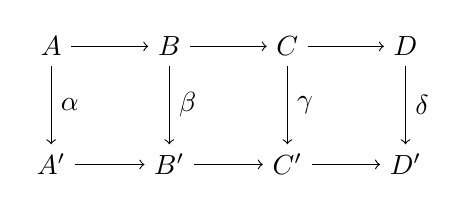
\begin{tikzpicture}[node distance=1.5cm, auto]
  \node (A) {$A$};
  \node (B) [right of=A] {$B$};
  \node (C) [right of=B] {$C$};
  \node (D) [right of=C] {$D$};
  \node (A') [below of=A] {$A'$};
  \node (B') [below of=B] {$B'$};
  \node (C') [below of=C] {$C'$};
  \node (D') [below of=D] {$D'$};

  \draw[->] (A) to (B);
  \draw[->] (B) to (C);
  \draw[->] (C) to (D);
  \draw[->] (A') to (B');
  \draw[->] (B') to (C');
  \draw[->] (C') to (D');

  \draw[->] (A) to node {$\alpha$} (A');
  \draw[->] (B) to node {$\beta$} (B');
  \draw[->] (C) to node {$\gamma$} (C');
  \draw[->] (D) to node {$\delta$} (D');
\end{tikzpicture}
\end{center}
is a commutative diagram of groups (you may assume the groups are abelian, if you find this psychologically helpful---it won't make a difference), and that the rows are exact (that is, the diagrams $A \rightarrow B \rightarrow C$, $B \rightarrow C \rightarrow D$, $A' \rightarrow B' \rightarrow C'$, $B' \rightarrow C' \rightarrow D'$ are exact at $B$, $C$, $B'$, $C'$ respectively).  Prove that

(a) if $\alpha$ is surjective, and $\beta$ and $\delta$ are injective, then $\gamma$ is injective;

\begin{proof}
Let the maps be $\psi: A \rightarrow B$, $\varphi: B \rightarrow C$, $\theta : C \rightarrow D$, $\psi ': A' \rightarrow B'$, $\varphi ': B' \rightarrow C'$, and $\theta ' : C' \rightarrow D'$.  Suppose $c \in \ker(\gamma)$, so the $\gamma(c) = 1$.

By commutativity, we have $\delta \circ \theta ( c) = \theta' \circ \gamma (c) = 1$, thus $\theta(c) = 1$ because $\delta$ is injective.  So $c \in \ker (\theta) = \im (\varphi)$ by exactness.  So there exists $b \in B$ such that $\varphi(b) = c$.

By commutativity, we have $\varphi ' \circ \beta (b) = \gamma \circ \varphi (b) = \gamma (c) = 1$.  Thus $\beta(b) \in \ker (\varphi ') = \im (\psi ')$, by exactness.  So there exists $a' \in A'$ such that $\psi ' (a') = \beta(b)$.

$\alpha$ is surjective, so there exists $a \in A$ such that $\alpha(a) = a'$.  So $\psi' \circ \alpha(a) = \psi'(a') = \beta(b)$.  By commutativity, we have $\beta \circ \psi (a) = \psi' \circ \alpha(a) = \beta(b)$.  Since $\beta$ is injective, this means $\psi(a) = b$.

By this last fact, $b \in \im (\psi) = \ker(\phi)$, so $\phi(b) = 1$.  $b$ was defined so that $\phi(b) = c$, thus $c = 1$.  So $\gamma$ is injective.
\end{proof}

(b) if $\delta$ is injective, and $\alpha$ and $\gamma$ are surjective, then $\beta$ is surjective.

\begin{proof}
Let $b' \in B'$.  Since $\gamma$ is surjective, there exists $c \in C$ such that $\gamma(c) = \varphi '(b')$.  So $\gamma(c) \in \im (\varphi') = \ker (\theta')$, thus $\theta'(\gamma(c)) = 1$.  By commutativity, $\delta(\theta(c)) = \theta'(\gamma(c)) = 1$.

$\delta$ is injective, so $\theta(c) = 1$.  So $c \in \ker (\theta) = \im(\varphi)$, by exactness, thus there exists $b \in B$ such that $\varphi(b) = c$.

By commutativity, $\varphi'(\beta(b)) = \gamma(\varphi(b)) = \gamma(c) = \varphi'(b')$.  So $\varphi'(\beta(b))\cdot (\varphi'(b'))^{-1} = \varphi'(\beta(b) \cdot (b')^{-1}) = 1$.  Hence, $\beta(b) \cdot (b')^{-1} \in \ker \varphi' = \im(\psi')$, so there exists $a' \in A'$ such that $\psi'(a') = \beta(b) \cdot (b')^{-1}$.

Since $\alpha$ is surjective, there exists $a \in A$ such that $\alpha(a) = a'$.  By exactness, $\beta(\psi(a)) = \psi'(\alpha(a)) = \psi'(a') = \beta(b) \cdot (b')^{-1}$.  So $b' = \beta(\psi(a))^{-1} \cdot \beta(b) = \beta(\psi(a^{-1})\cdot b)$.  Therefore, $\beta$ is surjective.
\end{proof}

\item (Exercise 12 in DF \S 10.5.) Let $A$ be an $R$-module, let $I$ be any nonempty index set, and for each $i \in I$ let $B_i$ be an $R$-module.  Prove that we have the following $R$-module isomorphisms:

(a) $\Hom_R(\bigoplus_{i \in I} B_i, A) \cong \prod_{i \in I} \Hom_R(B_i,A)$;

\begin{proof}
Define a map $\varphi: \Hom_R(\bigoplus_{i \in I} B_i, A) \rightarrow \prod_{i \in I} \Hom_R(B_i,A)$ as follows:

Let $f \in \Hom_R(\bigoplus_{i \in I} B_i, A)$.  For each $i \in I$, the map $f \circ \iota_i$ gives a homomorphism from $B_i$ to $A$, where $\iota_i$ is the natural inclusion of $B_i$ into $\bigoplus_{i \in I} B_i$.  So let $\varphi(f)$ be $\prod f \circ \iota_i \in \prod_{i \in I} \Hom_R(B_i,A)$.

%This is not a use of a universal property.  $\prod_{i \in I} \Hom_R(B_i,A)$ is not technically a set of maps; it is a direct product of sets of maps.  Its elements look like those of $\Hom_R(\prod_{i \in I}B_i,\prod_{i \in I}A)$, but these modules are not technically equal.

We will show that $\varphi$ is injective.  Suppose $\varphi(f) = 0$.  Then $\prod f \circ \iota_i = 0$, thus $f \circ \iota_i = 0$ for each $i \in I$.  Let $x \in \bigoplus_{i \in I} B_i$.  Since this is a direct sum, $x$ can be expressed as $x = \sum_{j \in J} \iota_j(b_j)$, where $J$ is some finite subset of $I$ and $b_j \in B_j$ for each $j \in J$.  Thus,
\begin{align*}
f(x) &= f(\sum_{j \in J} \iota_j(b_j))
\\
&= \sum_{j \in J} f \circ \iota_j(b_j)
\\
&= \sum_{j \in J} 0
\\
&= 0
\end{align*}
so $f$ is the zero map, thus $\varphi$ is injective.

Now, let $\prod g_i \in \prod_{i \in I} \Hom_R(B_i,A)$, where $g_i: B_i \rightarrow A$ for each $i \in I$.  We will show that $g$ is the image of $f$ under $\varphi$, where $f: \bigoplus_{i \in I} B_i \rightarrow A$ is the map given by $f(\sum_{j \in J} \iota_j(b_j)) = \sum_{j \in J} g_j(b_j)$ for any finite subset $J$ of $I$ where $b_j \in B_j$ for each $j \in J$ (again, every element of the direct sum is of this form).

To show that $\varphi(f) = \prod f \circ \iota_i$ equals $\prod g_i$, all we need to show is that $f \circ \iota_i = g_i$ for each $i \in I$.  But this is clear, since for any $x \in B_i$ we have defined $f$ so that $f \circ \iota_i(x) = g_i(x)$.  Thus $\varphi$ is surjective, therefore an isomorphism.
\end{proof}

(b) $\Hom_R(A, \prod_{i \in I} B_i) \cong \prod_{i \in I} \Hom_R(A,B_i)$.

\begin{proof}
Define $\varphi:\Hom_R(A, \prod_{i \in I} B_i) \rightarrow \prod_{i \in I} \Hom_R(A,B_i)$ by $\varphi(f) = \prod \pi_i \circ f$.

$\varphi$ is clearly injective.  If $f(x) \neq 0$ for some $x \in A$, then $\pi \circ f(x) \neq 0$ for some $i \in I$, thus $\varphi(f) = \prod \pi_i \circ f \neq 0$, so $f \not \in \ker (\varphi)$.

Now let $\prod g_i \in \prod_{i \in i} \Hom_R(A,B_i)$, where $g_i : A \rightarrow B_i$ for each $i \in I$.  Let $f: A \rightarrow \prod_{i \in I} B_i$ be defined by $f(x) = \prod g_i(x)$.  Then for any $x \in A$, we have 
\begin{align*}
\varphi(f)
&=
\prod \pi_i \circ f 
\\
&=\prod \pi_i \circ \prod g_j
\\
&= \prod g_i
\end{align*}
therefore $\varphi(f) = g$.  So $\varphi$ is surjective, thus an isomorphism.
\end{proof}

\end{enumerate}
\end{document}







